\chapter{Management Approach}

\section{Project Process}
The Agile Model was primarily designed to help a project adapt quickly to change requests. So, the main aim of the Agile model is to facilitate quick project completion. To accomplish this task, agility is required. Agility is achieved by fitting the process to the project and removing activities that may not be essential for a specific project. Also, anything that is a waste of time and effort is avoided. The Agile Model refers to a group of development processes.

\textbf{\large Agile SDLC Models/Methods}\\
\textbf{Given below are some Agile SDLC Models:}
\begin{itemize}
    \item Crystal Agile methodology: The Crystal Agile Software Development Methodology places a strong emphasis on fostering effective communication and collaboration among team members, as well as taking into account the human elements that are crucial for a successful development process. This methodology is particularly beneficial for projects with a high degree of uncertainty, where requirements tend to change frequently.
    
    \item Dynamic Systems Development Method (DSDM): DSDSM methodology is tailored for projects with moderate to high uncertainty where requirements are prone to change frequently. Its clear-cut roles and responsibilities focus on delivering working software in short time frames. Governance practices set it apart and make it an effective approach for teams and projects.
    
    \item Feature-driven development (FDD): FDD approach is implemented by utilizing a series of techniques, like creating feature lists, conducting model evaluations, and implementing a design-by-feature method, to meet its goal. This methodology is particularly effective in ensuring that the end product is delivered on time and that it aligns with the requirements of the customer.

    \item Scrum: Scrum methodology serves as a framework for tackling complex projects and ensuring their successful completion. It is led by a Scrum Master, who oversees the process, and a Product Owner, who establishes the priorities. The Development Team, accountable for delivering the software, is another key player.

    \item Extreme Programming (XP): Extreme Programming uses specific practices like pair programming, continuous integration, and test-driven development to achieve these goals. Extreme programming is ideal for projects that have high levels of uncertainty and require frequent changes, as it allows for quick adaptation to new requirements and feedback.

    \item Lean Development: Lean Development is rooted in the principles of lean manufacturing and aims to streamline the process by identifying and removing unnecessary steps and activities. This is achieved through practices such as continuous improvement, visual management, and value stream mapping, which helps in identifying areas of improvement and implementing changes accordingly. 

    \item Unified Process: Unified Process is a methodology that can be tailored to the specific needs of any given project. It combines elements of both waterfall and Agile methodologies, allowing for an iterative and incremental approach to development. This means that the UP is characterized by a series of iterations, each of which results in a working product increment, allowing for continuous improvement and the delivery of value to the customer.
\end{itemize}

All Agile Software Development Methodology discussed above share the same core values and principles, but they may differ in their implementation and specific practices. Agile development requires a high degree of collaboration and communication among team members, as well as a willingness to adapt to changing requirements and feedback from customers.

In the Agile model, the requirements are decomposed into many small parts that can be incrementally developed. The Agile model adopts Iterative development. Each incremental part is developed over an iteration. Each iteration is intended to be small and easily manageable and can be completed within a couple of weeks only. At a time one iteration is planned, developed, and deployed to the customers. Long-term plans are not made. 

\textbf{Steps in the Agile Model}
The agile model is a combination of iterative and incremental process models. The steps involve in agile SDLC models are: 
\begin{itemize}
    \item Requirement gathering
    \item Design the Requirements
    \item Construction / Iteration
    \item Testing / Quality Assurance
    \item Deployment
    \item Feedback
\end{itemize}


\begin{figure}
    \centering
    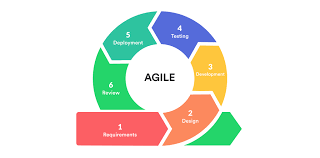
\includegraphics[width=1\linewidth]{images/agile-process-model.png}
    \caption{Agile process model}
    \label{fig:agile-process-model}
\end{figure}


\begin{itemize}
    \item Requirement Gathering:- In this step, the development team must gather the requirements, by interaction with the customer. development team should plan the time and effort needed to build the project. Based on this information you can evaluate technical and economical feasibility.

    \item Design the Requirements:- In this step, the development team will use user-flow-diagram or high-level UML diagrams to show the working of the new features and show how they will apply to the existing software. Wireframing and designing user interfaces are done in this phase.

    \item Construction / Iteration:- In this step, development team members start working on their project, which aims to deploy a working product.

    \item Testing / Quality Assurance:- Testing involves Unit Testing, Integration Testing, and System Testing. A brief introduction of these three tests is as follows:
    \begin{itemize}
        \item Unit Testing:- Unit testing is the process of checking small pieces of code to ensure that the individual parts of a program work properly on their own. Unit testing is used to test individual blocks (units) of code.
        \item Integration Testing:- Integration testing is used to identify and resolve any issues that may arise when different units of the software are combined.
        \item System Testing:- Goal is to ensure that the software meets the requirements of the users and that it works correctly in all possible scenarios.
    \end{itemize}

    \item Deployment:- In this step, the development team will deploy the working project to end users.

    \item Feedback:- This is the last step of the Agile Model. In this, the team receives feedback about the product and works on correcting bugs based on feedback provided by the customer.
\end{itemize}